Concerning the first of the objectives described in the Introduction chapter, no formal method is used to \emph{obtain} the ``vision'' of a future mobility system. The vision is not derived from any kind of forecasting or modelling tool. Instead, a literature review was performed at the beginning of the thesis, searching for papers with the keywords ``sustainable'', ``mobility'' and ``paradigm''. While several articles were found (e.g., \textcite{banister2008_sustainablemobilityparadigm}), little or none of them actually gave a clear picture of a \emph{future paradigm} of sustainable mobility. Most of the papers consisted only on discussions regarding some of the aspects that could conform a sustainable mobility paradigm. Therefore, the decision was taken to build a new vision on already existing research. The final choice for the basis of the vision is the long-term scenario framework by the \gls{IPCC} (see \sref{s:results:ssp1-mob} for more detail). This framework consists on five different qualitative narratives that are then translated into sets of (quantitative) assumptions in the global climate change assessment models (\gls{IAM}).

\begin{figure}
\centering
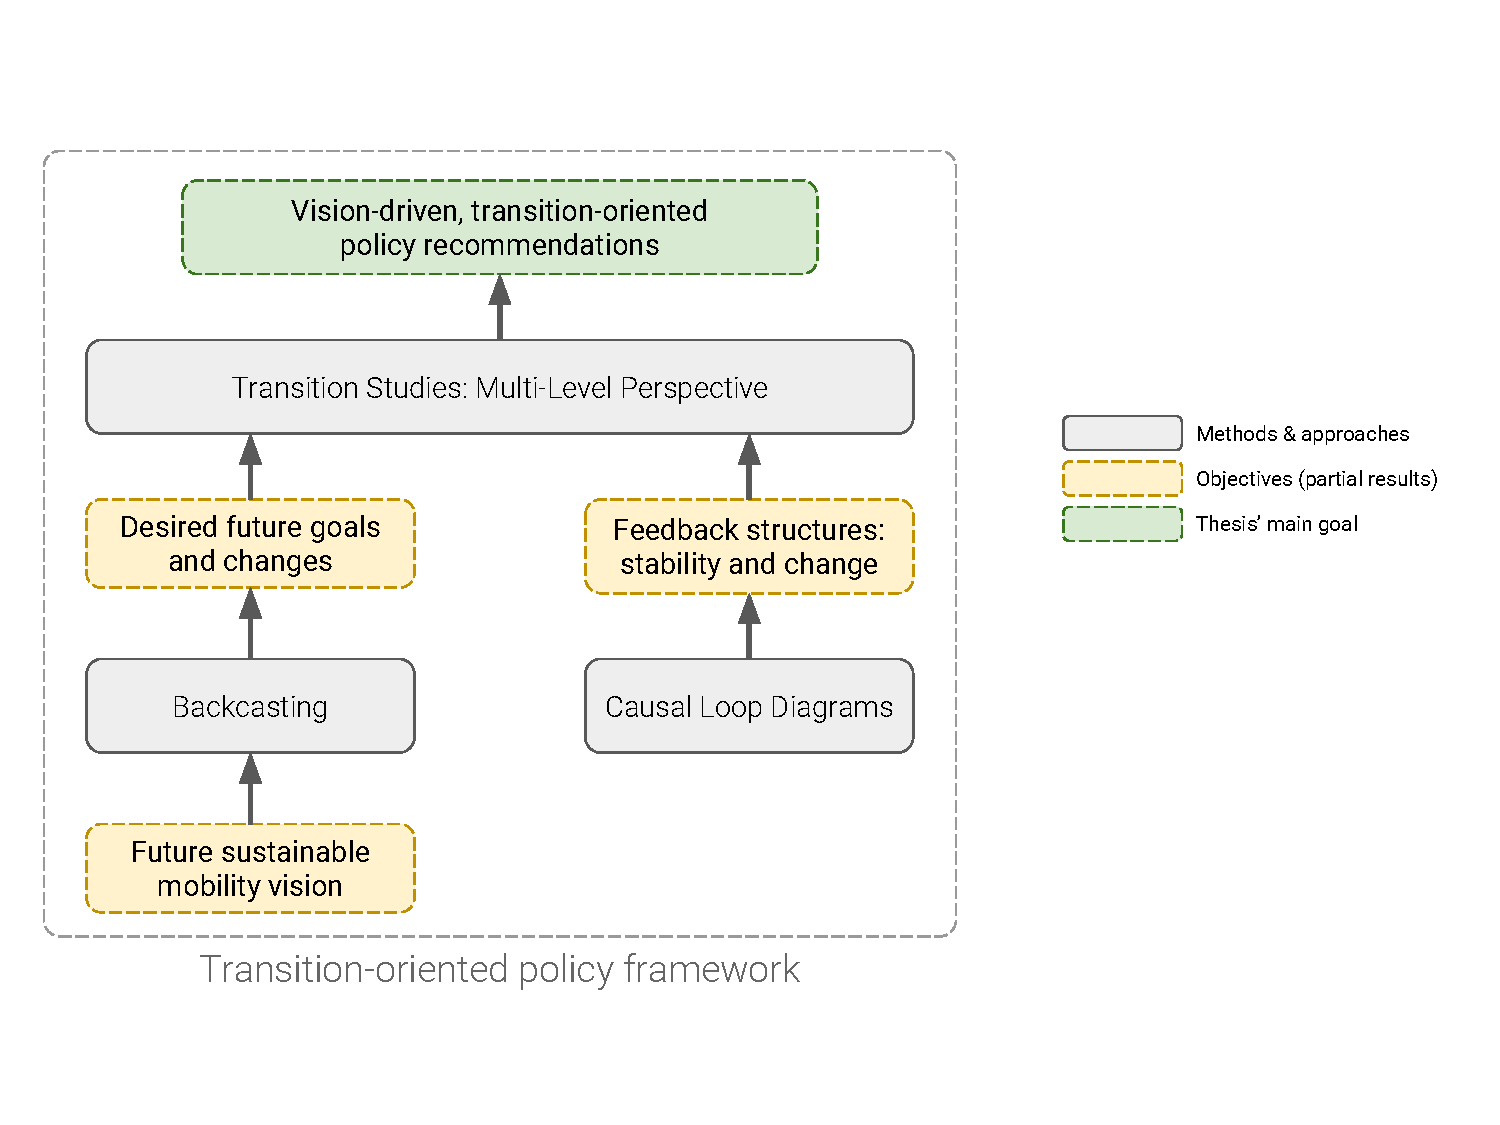
\includegraphics[width=0.8\linewidth,trim=0 2cm 0 2cm,clip]{figures/methods-goals.pdf}
\caption[Methodological framework]{Methodological framework, linking methods to objectives and showing the flow of information until the final aim (policy recommendations) is reached.}
\label{f:thesis-aim-methods}
\end{figure}

The vision in this thesis is developed following the same method as \textcite{oneill2017_roadsaheadNarratives} did for the IPCC scenarios: through a \emph{qualitative narrative} in which the aspects of the sustainable mobility paradigm are explained qualitatively. With respect to how the vision is developed, it is done so by building upon the foundations of the SSP1 scenario by the IPCC, in combination with insights gained from the literature. However, the structural elements of the narrative are withdrawn from the IPCC's storyline.

The fact that the IPCC scenarios are developed from a set of narratives actually makes them easier to transform into a ``vision'' than more traditional scenarios: the IPCC scenarios explore final \emph{states}, rather providing with forecasts. Drawing on the scenario typology built by \textcite{boerjeson2006_Scenariotypestechniques}, IPCC's would fall under the ``exploratory'' scenarios category, while the actual approach of the backcasting process (see \sref{s:methods:backcasting}) in this thesis would fall under the ``normative'' category. Despite these seem not to fit, the truth is that in order to build the vision for the backcasting in \ssref{ss:results:ssp1-mob-development}, it is very useful to start from the ground of an already developed, consistent and acknowledged exploration of a \emph{possible} future. This way, a lot of assumptions are already justified and the whole vision frame is not purely speculative in nature.